% Phase 2 network topology (build: tectonic phase2_topology.tex)
\documentclass[border=8pt]{standalone}
\usepackage[T1]{fontenc}
\usepackage{lmodern}
\usepackage{tikz}
\usetikzlibrary{positioning,arrows.meta,fit,backgrounds,calc}

\definecolor{navy}{HTML}{17365D}
\definecolor{dnsc}{HTML}{2E75B6}
\definecolor{edgec}{HTML}{C55A11}
\definecolor{appc}{HTML}{548235}
\definecolor{fwc}{HTML}{C00000}
\definecolor{clic}{HTML}{7F6000}
\definecolor{lan}{HTML}{F2F2F2}

\tikzset{
  vm/.style={draw=#1, line width=0.9pt, rounded corners=3pt, fill=#1!8,
             minimum width=5.0cm, minimum height=1.55cm, align=center, font=\small},
  svc/.style={draw=#1, line width=0.6pt, rounded corners=2pt, fill=white,
              minimum width=2.25cm, minimum height=0.62cm, align=center, font=\scriptsize},
  flow/.style={-{Stealth[length=2.6mm]}, line width=0.9pt, draw=#1},
  lbl/.style={font=\scriptsize, fill=white, inner sep=1.5pt, text=#1},
}

\begin{document}
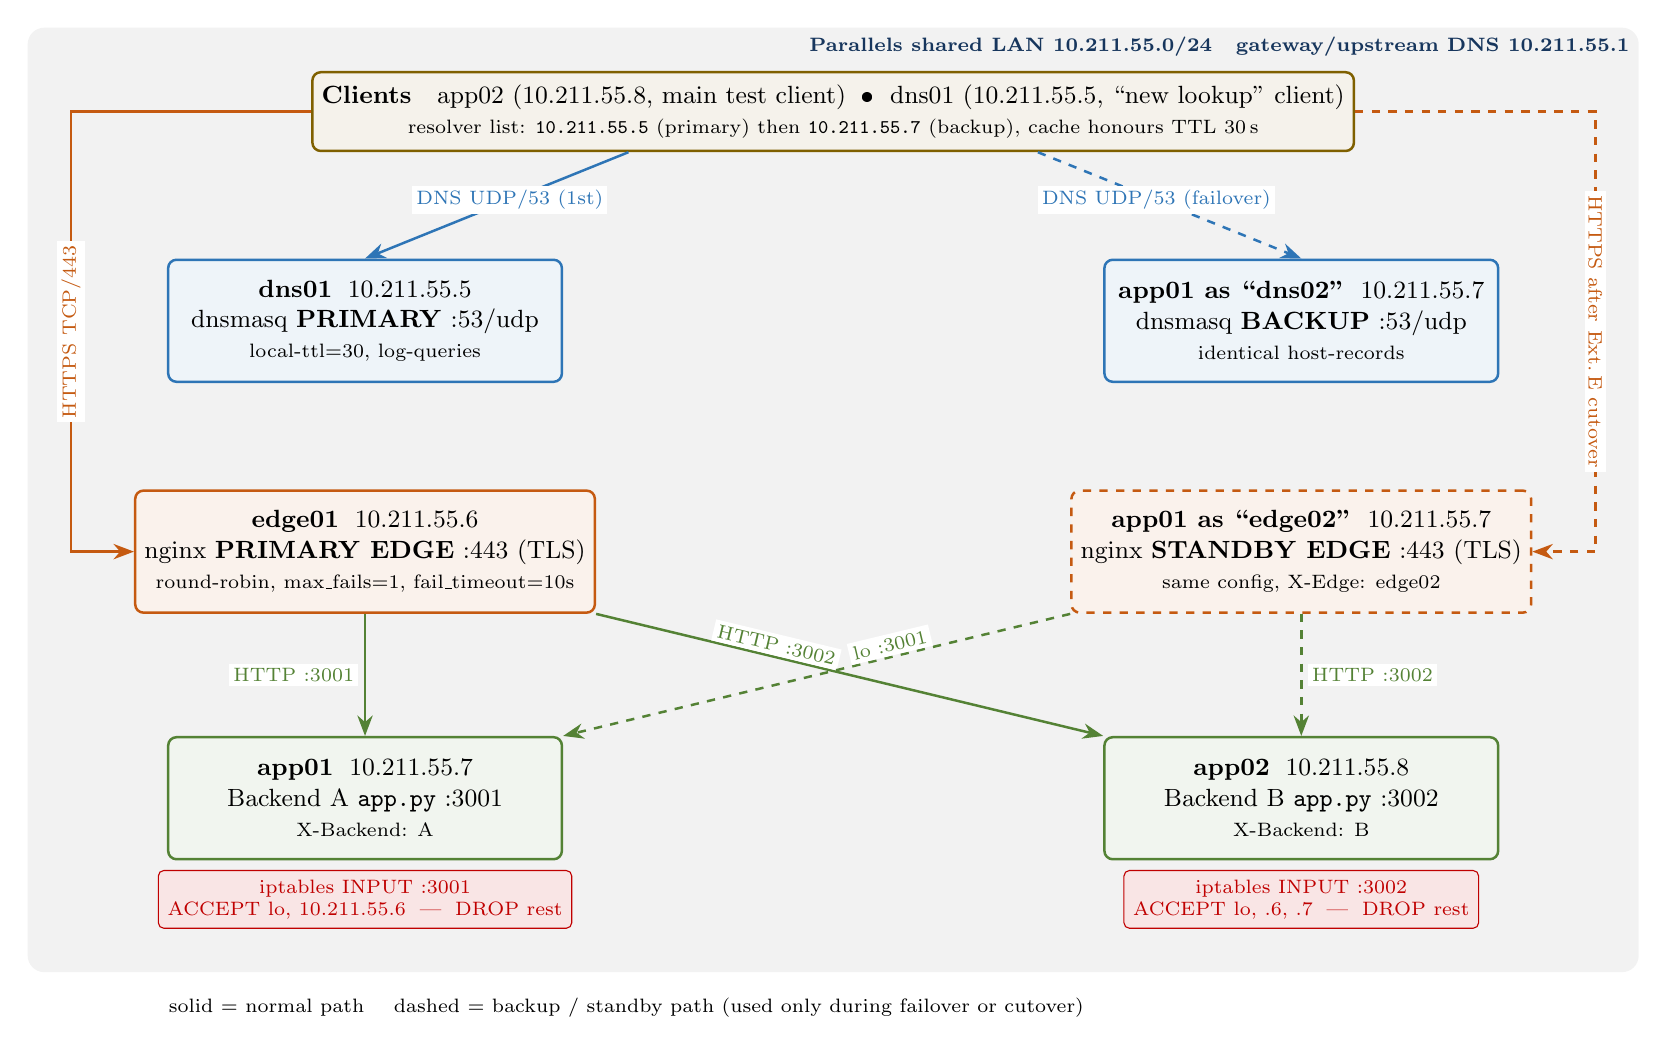
\begin{tikzpicture}[node distance=1.0cm and 1.1cm]

% ---------------- Clients ----------------
\node[vm=clic, minimum width=11.4cm, minimum height=1.0cm] (clients)
  {\textbf{Clients}\quad app02 (10.211.55.8, main test client) \;\textbullet\; dns01 (10.211.55.5, ``new lookup'' client)\\
   \scriptsize resolver list: \texttt{10.211.55.5} (primary) then \texttt{10.211.55.7} (backup), cache honours TTL 30\,s};

% ---------------- DNS tier ----------------
\node[vm=dnsc, below left=1.35cm and -3.2cm of clients] (dns01)
  {\textbf{dns01}\; 10.211.55.5\\ dnsmasq \textbf{PRIMARY} :53/udp\\ \scriptsize local-ttl=30, log-queries};
\node[vm=dnsc, below right=1.35cm and -3.2cm of clients] (dns02)
  {\textbf{app01 as ``dns02''}\; 10.211.55.7\\ dnsmasq \textbf{BACKUP} :53/udp\\ \scriptsize identical host-records};

% ---------------- Edge tier ----------------
\node[vm=edgec, below=1.35cm of dns01] (edge01)
  {\textbf{edge01}\; 10.211.55.6\\ nginx \textbf{PRIMARY EDGE} :443 (TLS)\\ \scriptsize round-robin, max\_fails=1, fail\_timeout=10s};
\node[vm=edgec, below=1.35cm of dns02, dashed] (edge02)
  {\textbf{app01 as ``edge02''}\; 10.211.55.7\\ nginx \textbf{STANDBY EDGE} :443 (TLS)\\ \scriptsize same config, X-Edge: edge02};

% ---------------- Backend tier ----------------
\node[vm=appc, below=1.55cm of edge01] (appA)
  {\textbf{app01}\; 10.211.55.7\\ Backend A \texttt{app.py} :3001\\ \scriptsize X-Backend: A};
\node[vm=appc, below=1.55cm of edge02] (appB)
  {\textbf{app02}\; 10.211.55.8\\ Backend B \texttt{app.py} :3002\\ \scriptsize X-Backend: B};

% Firewall badges
\node[draw=fwc, fill=fwc!10, rounded corners=2pt, font=\scriptsize, text=fwc, align=center, anchor=north] (fwA)
  at ($(appA.south)+(0,-0.12)$) {iptables INPUT :3001\\ ACCEPT lo, 10.211.55.6 \;|\; DROP rest};
\node[draw=fwc, fill=fwc!10, rounded corners=2pt, font=\scriptsize, text=fwc, align=center, anchor=north] (fwB)
  at ($(appB.south)+(0,-0.12)$) {iptables INPUT :3002\\ ACCEPT lo, .6, .7 \;|\; DROP rest};

% ---------------- Flows ----------------
\draw[flow=dnsc] ($(clients.south)+(-2.6,0)$) -- node[lbl=dnsc, pos=0.45] {DNS UDP/53 (1st)} (dns01.north);
\draw[flow=dnsc, dashed] ($(clients.south)+(2.6,0)$) -- node[lbl=dnsc, pos=0.45] {DNS UDP/53 (failover)} (dns02.north);

\coordinate (lx) at ($(edge01.west)+(-0.8,0)$);
\coordinate (rx) at ($(edge02.east)+(0.8,0)$);
\draw[flow=edgec] (clients.west) -| (lx |- clients.west) -- node[lbl=edgec, midway, rotate=90] {HTTPS TCP/443} (lx) -- (edge01.west);
\draw[flow=edgec, dashed] (clients.east) -| (rx |- clients.east) -- node[lbl=edgec, midway, rotate=-90] {HTTPS after Ext.\,E cutover} (rx) -- (edge02.east);

\draw[flow=appc] (edge01.south) -- node[lbl=appc, left=2pt] {HTTP :3001} (appA.north);
\draw[flow=appc] (edge01.south east) -- node[lbl=appc, pos=0.35, sloped, above] {HTTP :3002} (appB.north west);
\draw[flow=appc, dashed] (edge02.south west) -- node[lbl=appc, pos=0.35, sloped, above] {lo :3001} (appA.north east);
\draw[flow=appc, dashed] (edge02.south) -- node[lbl=appc, right=2pt] {HTTP :3002} (appB.north);

% LAN background
\begin{scope}[on background layer]
  \node[fill=lan, rounded corners=6pt, inner sep=0.55cm, fit=(clients)(dns01)(dns02)(edge01)(edge02)(appA)(appB)(fwA)(fwB)(lx)(rx),
        label={[font=\scriptsize\bfseries, text=navy, anchor=north east]north east:Parallels shared LAN 10.211.55.0/24 \; gateway/upstream DNS 10.211.55.1}] {};
\end{scope}

% Legend
\node[font=\scriptsize, align=left, anchor=north west] at ($(fwA.south -| appA.west)+(-0.1,-0.75)$)
  {solid = normal path \quad dashed = backup / standby path (used only during failover or cutover)};

\end{tikzpicture}
\end{document}
